\begin{frame}
\begin{block}{diagram}
Let $\mathcal{C}$ be a category. A {\it diagram} in $\mathcal{C}$ is a functor $M : \mathcal{I} \to \mathcal{C}$. $\mathcal{I}$ is the {\it index category} and $M$ is an $\mathcal{I}$-diagram. $M_i$ denotes the image of the object $i$ of $\mathcal{I}$ in $\cC$. For $\phi : i \to i' \in \Mor(I)$, $M(\phi) : M_i \to M_{i'}$.
\end{block}
\begin{block}{}
\centering 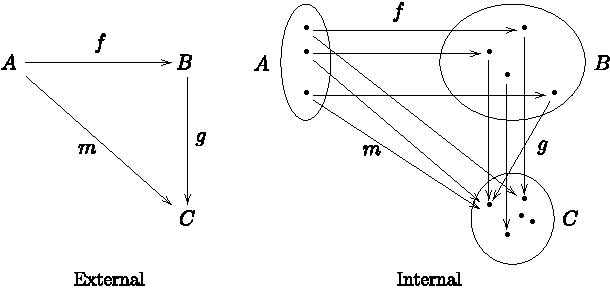
\includegraphics[width=0.7\textwidth]{fig/intextdiag.pdf}
\end{block}
\end{frame}